\documentclass[12pt]{article}

\usepackage[utf8]{inputenc}
\usepackage[left=2cm,right=2cm,top=2cm,bottom=4cm]{geometry}
\usepackage[ngerman]{babel}
\usepackage{amsmath, amsfonts, amssymb, amsthm}
\usepackage{graphicx}
\usepackage{multicol}
\usepackage[compact]{titlesec}

\usepackage{ulem, contour}
\usepackage{xcolor, colortbl}
\usepackage{caption, subcaption}
\usepackage{listings}
\usepackage{hyperref}

\renewcommand{\ULdepth}{1.8pt}
\contourlength{0.8pt}
\newcommand{\cul}[1]{%
  \uline{\phantom{#1}}%
  \llap{\contour{white}{#1}}%
}

\lstset{
    language=tex,
    backgroundcolor=\color{black!5},
    basicstyle=\footnotesize,
}

\theoremstyle{definition}
\newtheorem*{definition}{Definition}
\newtheorem*{example}{Beispiel}

\definecolor{darkgreen}{rgb}{0.0, 0.3, 0.15}

\begin{document}

\section{Ablauf des Programms}

\begin{flushleft}
\begin{enumerate}
\item[Schritt 1:] Zuerst wird die Kamera mit dem Python-script gestartet. Sie nimmt kontinuierlich auf und sendet das Bild zur weiterverarbeitung an das Skript.

\item[Schritt 2:] Sobald die Kamera einen Input erhält (also aufnimmt) wird über die Frames iteriert. Dabei wird jeder Frame einzeln betrachtet.

\item[Schritt 3:] Der Frame wird nun mit der pre-trained Tensorflow Erkennungs-KI predictet. Ist auf dem Frame ein Objekt, für das trainiert wurde\footnote{Alle erkennbaren Objekte sind in der labelmap \textit{Sample\_Model/labelmap.txt} gelistet}, zu erkennen werden der Score (Treffsicherheit), die Klasse (Objektbezeichnung) und Koordinaten (obere linke Ecke und untere rechte Ecke) des Objektes gespeichert.

\item[Schritt 4:] Nachdem der Frame predictet wurde, wird um jedes erkannte Objekt eine farbige Box gezeichnet, um es zu markieren. Hierbei kann ggf. nach Objekten gefiltert werden, z.B. nach 'person' um nur Personen zu markieren. Für eine bessere Sichtbarkeit und bessere Übersicht wurde ein Farbwechsel für die Boxen implementiert. Hierbei sind sechs Grün- und Rottöne vorhanden, wodurch 36 verschiedene Farben möglich sind. Dies lässt sich bei Bedarf aber auch erhöhen.

\begin{figure}[h]
\begin{subfigure}[t]{0.5\textwidth}
	\centering
	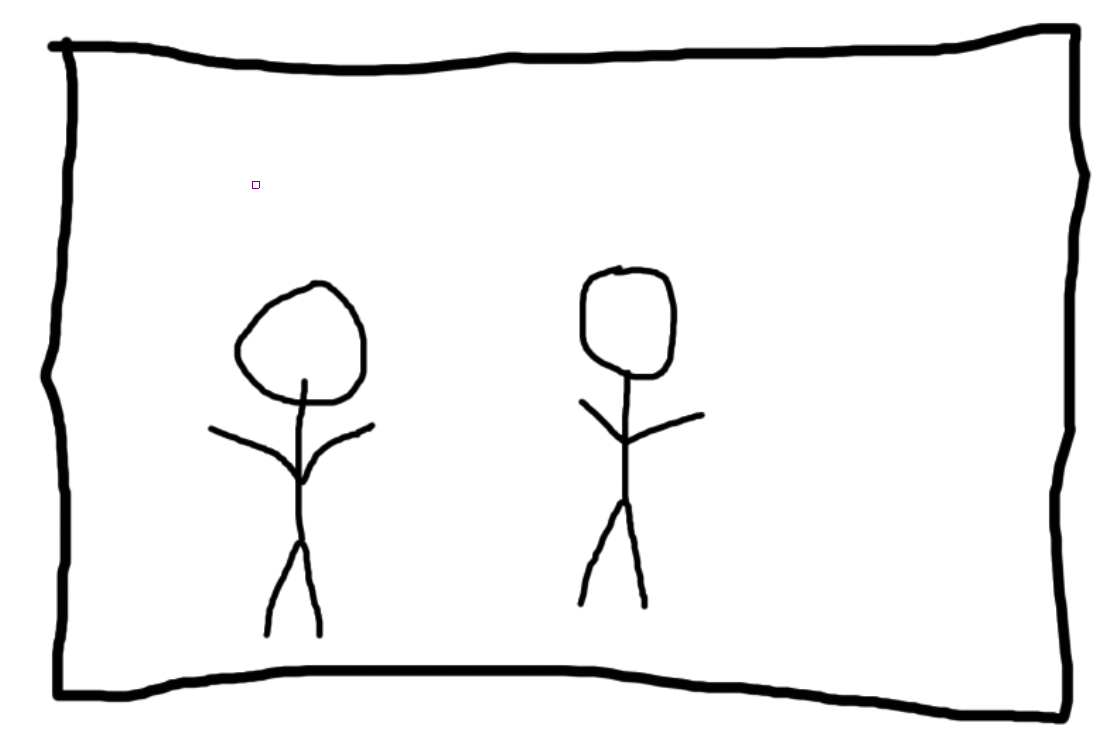
\includegraphics[scale=0.25]{step0.png}
	\subcaption*{Schritt 3: Ein Frame}
\end{subfigure}%
\begin{subfigure}[t]{0.5\textwidth}
	\centering
	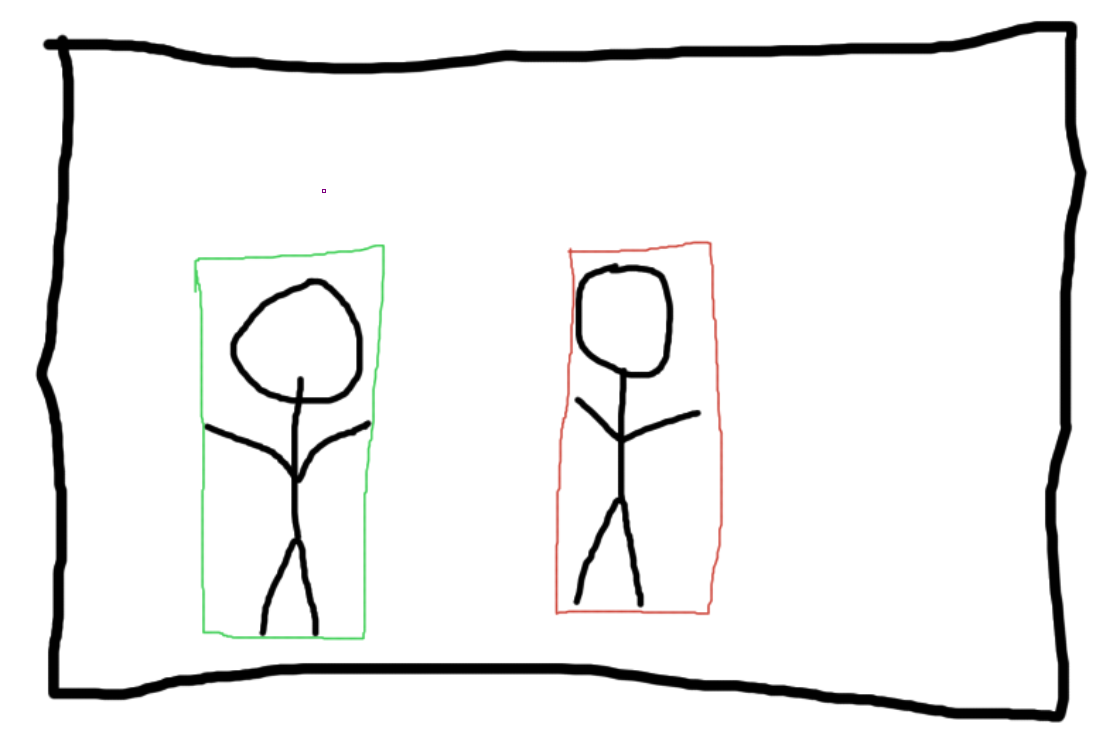
\includegraphics[scale=0.25]{step1.png}
	\subcaption*{Schritt 4: Boxen um Objekte}
\end{subfigure}%
\end{figure}

\item[Schritt 5:] Zusätzlich zu den Markierungen wird auch der Abstand zwischen jeweils zwei Objekten gemessen. Hierbei wird der relative Abstand auf approximativer Basis mit Hilfe der Durchschnittswerte für Körpermaße bestimmt. Dadurch kann u.a. approximativ gut bestimmt werden, wie viele Pixel ein Zentimeter ergeben. Aus der bekannten Breite der Person kann dann der Abstand zu Kamera ermittelt werden, sowie der horizontale Abstand der beiden Personen / Objekte.

\item[Schritt 6:] Nachdem alles kalkuliert wurde, wird geprüft, ob der berechnete Abstand dem Mindestabstand genügt. Wenn nicht, wird eine Linie zwischen den Objekten gezeichnet, die zeigt, dass der Abstand zu gering ist. Zusätzlich wird der aktuell ermittelte Abstand angezeigt, sowie der benötigte Abstand.

\begin{figure}[h]
\begin{subfigure}[t]{0.5\textwidth}
	\centering
	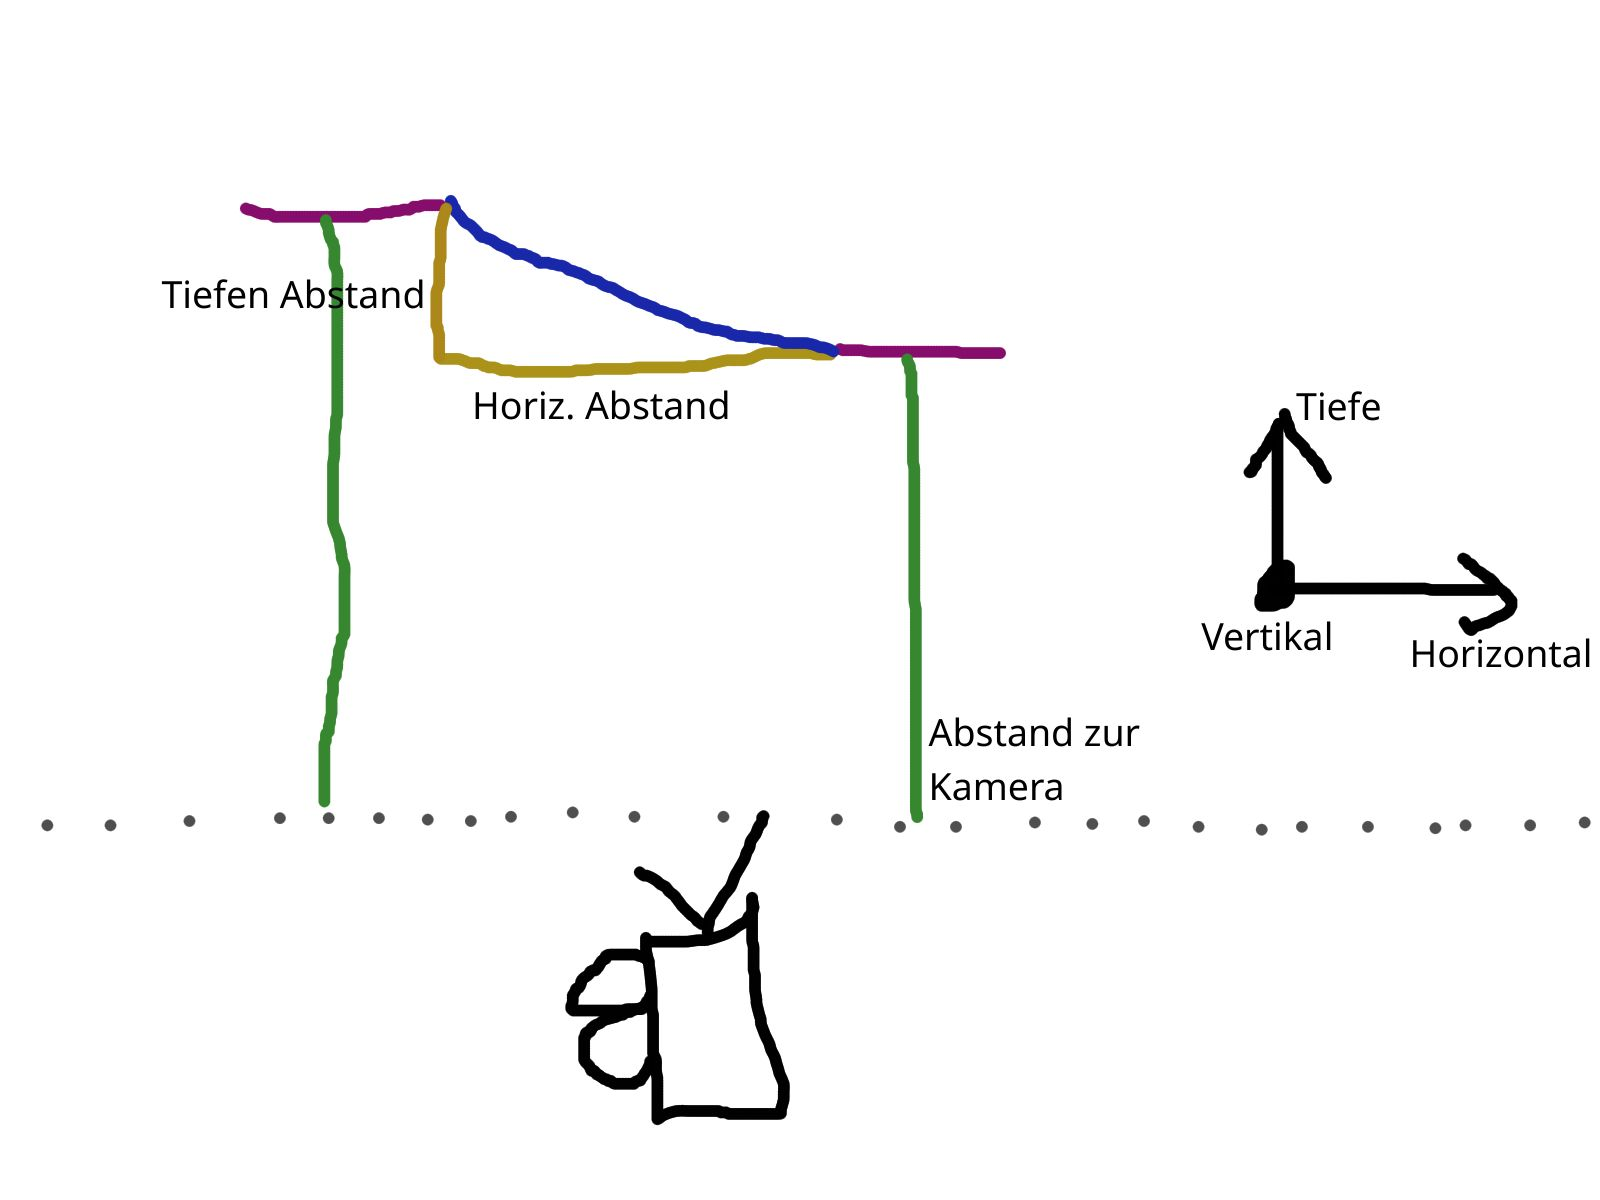
\includegraphics[scale=0.45]{Abstand_kalk.jpg}
	\subcaption*{Schritt 5: Berechnungen veranschaulicht}
\end{subfigure}%
\begin{subfigure}[t]{0.5\textwidth}
	\centering
	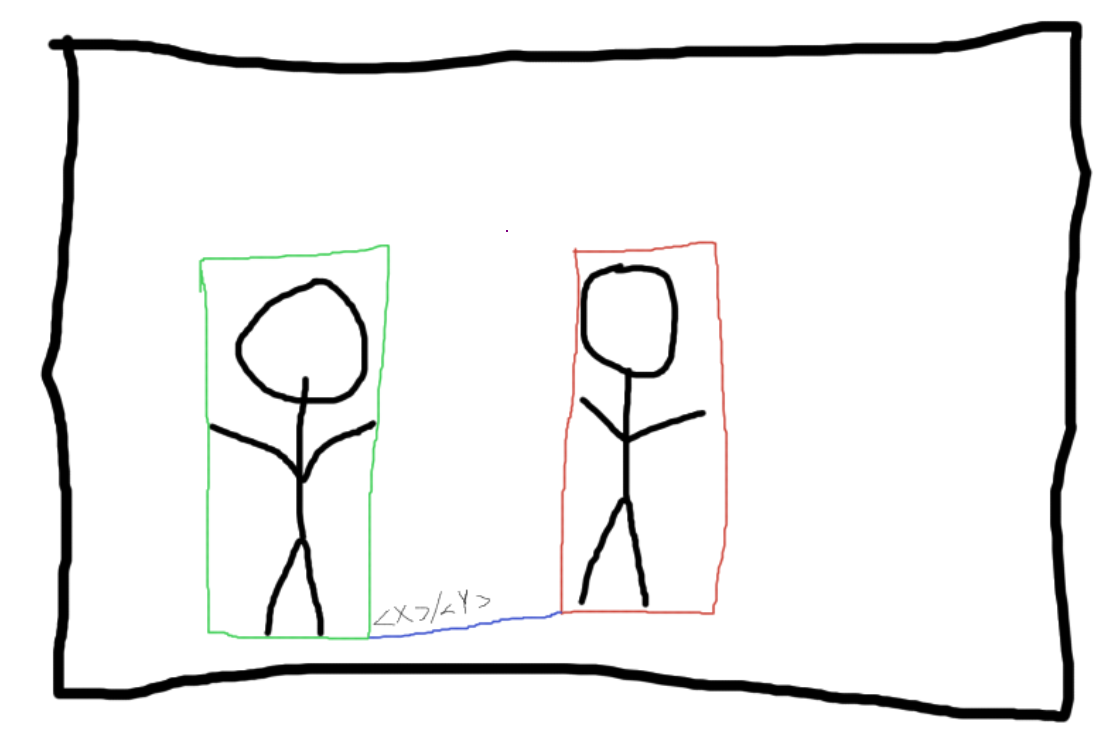
\includegraphics[scale=0.25]{step3.png}
	\subcaption*{Schritt 6: Abstandslinie}
\end{subfigure}%
\end{figure}

\item[Schritt 7:] Wiederhole Schritt 3 und folgende, bis das Programm beendet wird (Zum beenden drücke \textit{q}).
\end{enumerate}
\end{flushleft}

\section{Informationen}

\begin{flushleft}
Für die Berechnungen des Programms werden u.a. Durchschnittswerte genutzt. Hierbei wird für die durchschnittliche Breite einer Person der Wert 45 Zentimeter genutzt, wobei zehn Zentimeter addiert werden, da die Box meist über die Schulterbreite hinaus geht.

Um den Abstand eines Objektes zur Kamera zu berechnen, ist es notwendig den Fokalwert der Kameralinse zu wissen. Der Zusammenhang zwischen Abstand und Fokalwert zeigt sich in der Formel $F = \frac{P \cdot D}{W}$, wobei F der Fokalwert, P die Objektbreite in Pixel, D der Abstand des Objektes zur Kamera und W die Objektbreite in einer Maßeinheit\footnote{Wir verwenden hauptsächlich Zentimeter} ist.
\end{flushleft}

\end{document}